\chapter{Ontwerp van het project}
\label{hoofdstuk:ontwerp}

Eenmaal de belangrijkste vereisten gekend zijn kan er een ontwerp opgetekend worden. Daarom even de grote lijnen die te concluderen vallen uit hoofdstuk \ref{hoofdstuk:doelen}:

\begin{itemize}
  \item De data en het visuele aspect van de applicatie moeten zo ontkoppeld mogelijk zijn, elk moet apart uitbreidbaar zijn
  \item Zeer grote hoeveelheden data moeten vlot kunnen behandeld en genavigeerd worden: zoeken, filteren, sorteren, aanpassen, \ldots
  \item De data moet zowel centraal als decentraal toegankelijk zijn en synchronisatie toestaan
  \item Compatibiliteit met de reeds geschreven onderdelen van het project moet indien mogelijk bewaard blijven
  \item Om het ontwerp te verifi\"eren moet een werkend programma gemaakt worden, gebruiksvriendelijkheid, functionaliteit en snelheid zijn hierbij belangrijk
\end{itemize}

\section{De grote lijnen}
Van alle vereisten die rechtstreeks invloed kunnen uitoefenen op de architectuur, is de splitsing van de data en de visualisatie waarschijnlijk de meest fundamentele. Een beproefde aanpak om dit te realizeren is het ontwerppatroon genaamd \emph{Model-View-Controller (MVC)}\footnote{Een algemeen overzicht kan men bijvoorbeeld bekomen op \url{http://en.wikipedia.org/wiki/Model-view-controller}}.\\

Het doel is een ontwerp te maken waarin elke verschillende visualisatiemethode kan verbonden worden aan een geschikte databron, wat die ook moge zijn. Enkele zaken moeten echter nog vastgelegd worden, namelijk: wat is de basiseenheid van data? Waar zal een visualisatiemodule achter vragen? Zoals in figuur~\ref{fig:flow} te zien is, ligt de focus bij dit project op koppelingen van fragmenten in plaats van fragmenten op zich.\\

Er zijn op het eerste zicht twee alternatieven om dit te modelleren. De eerste mogelijkheid is een soort van \emph{MatchedFragment} die een fragment beschrijft plus een lijst met alle fragmenten die er potentieel aan gekoppeld kunnen worden en op welke locatie. De tweede mogelijkheid is om elk paar een apart object te laten voorstellen (bvb. genaamd \emph{FragmentPair}). Conceptueel kan dit gezien worden als een graaf, waarop de fragmenten de knopen voorstellen en de paren de zijden. Het eerste alternatief lijkt het voordeel te hebben dat het gemakkelijk is om na te kijken of een fragment reeds ``bezet'' is, alle mogelijke gekoppelde fragmenten zijn immers meteen beschikbaar. Echter, dit soort opstelling bevat op het eerste zicht veel redundantie, een fragment zal op die manier een verwijzing met attributen naar een fragment bevatten, en dit fragment zal op zijn beurt een identieke omgekeerde verbinding hebben. De redundantie vermijden en een verwijzing als een apart object voorstellen waar beide fragmenten naar kunnen verwijzen is eigenlijk niets anders dan de tweede optie (een \emph{FragmentPair}). Op die manier wordt de situatie omgedraaid en kan een fragmentenpaar verwijzen naar de fragmenten die het opbouwen. Daarbij kan het probleem van hoe de bezetting van een brokstuk te weten te komen opgelost worden door de vereiste zoekfunctionaliteit van het datamodel te benutten. Om die reden wordt ervoor gekozen om een fragmentpaar te gebruiken in plaats van een fragment met referenties naar alle buur fragmenten.\\

Eenmaal de basiseenheid van informatie gekozen is, valt de kern van de applicatie volgens MVC uit te beelden als in figuur~\ref{fig:basicprogramflow}.

\begin{figure}[ht]
	\begin{center}
		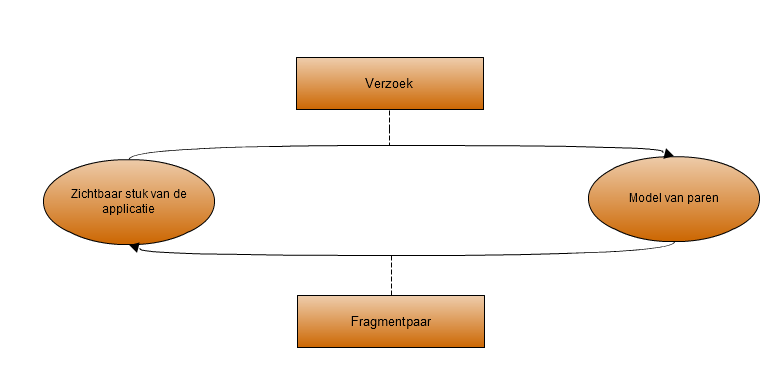
\includegraphics[width=1.0\columnwidth]{images/BasicExecutionFlow.png}
		\caption{Het abstracte model van de applicatie, links staat de \emph{View/Controller} en rechts het \emph{Model}. De controller stuurt een verzoek naar het model voor een bepaalde (sub)set van de data --- al dan niet gesorteerd --- en het model antwoord met alle paren die voldoen aan de criteria}
		\label{fig:basicprogramflow}
	\end{center}
\end{figure}

De gebruikersinterface en de achterliggende bibliotheken werden gemaakt met behulp van de Qt toolkit~\cite{qtdoc} in C++. Hierdoor is de applicatie te gebruiken op zowel UNIX als Windows systemen. Zoveel mogelijk zware berekeningen worden in parallel uitgevoerd, waardoor de applicatie snel opstart en responsief blijft, dit komt de gebruikerservaring ten goede.\\

\section{Modellen}
Een model is een abstracte voorstelling van een databron, het stelt de ontwikkelaar in staat om op een eenvoudige manier naar objecten te vragen en ze aan te passen zonder zich druk te hoeven maken over waar die vandaan komen. Dit is noodzakelijk om de nodige flexibiliteit te kunnen garanderen, zodat bijvoorbeeld een XML-bestand op de thuiscomputer plots kan ingewisseld worden voor een database kilometers verder zonder aan functionaliteit in te boeten.\\

Met enkele uitzonderingen handelt het type model gemaakt voor dit thesisproject enkel in fragmentparen. Op zijn minst bestaat zo'n paar uit twee fragmenten, een transformatie die beide fragmenten tegen elkaar plaatst en eventueel een resem attributen. De objecten die geproduceerd worden door de identificatiealgoritmen van het thera project voldoen reeds aan deze twee voorwaarden. Er bestaan al veel componenten die hiervan gebruik maken dus dezelfde interface recycleren bevordert de integratie met het moederproject.\\

De mogelijke operaties op een model kunnen in twee categorie\"en ondergebracht worden, opvragingen en aanpassingen. Vooral opvragingen zijn interessant omdat ze de ontwikkelaar en gebruiker in staat stellen hun eigen criteria te stellen over welke paren terugkomen. Een voorbeeld is: geef alle fragmentparen uit bak 33 van collectie WDC13 gerangschikt op dalende volumedoorsnede die als ``mogelijk correct'' te boek staan en commentaar hebben gekregen. Op die manier kan men snel navigeren naar de gewenste deelverzameling.

\subsection{Opvragen}
Het concept achter het opvragen van fragmentparen is dat er steeds wordt begonnen vanuit de volledige beschikbare verzameling die op het moment in de databron aanwezig is. De standaardoperaties zijn vervolgens \textbf{filteren} en \textbf{sorteren}. \\

Sorteren is eenvoudig en kan op eender welk attribuut in stijgende of dalende zin gebeuren. Filters gebruiken een krachtige syntax die volledig gelijk is aan die van de \emph{WHERE}-clausule van een SQL zin\footnote{SQL of Structured Query Language is een declaratieve taal om vragen te stellen aan een database. Er zijn vele verschillende implementaties die allen (bij benadering) dezelfde taal verstaan, men groepeert deze doorgaans onder de naam SQL databases.} (voorbeeld: broncode~\ref{code:sortingfiltering}). Visualisatiemodules kunnen indien gewenst geavanceerde gebruikers zelf filters laten verzinnen, maar veelgebruikte filter- en sorteeroperaties worden ook als knoppen en invoervelden blootgesteld, zoals in figuur~\ref{fig:tangfiltersort}.\\

De voorwaarde die aan filters gesteld wordt is dat ze enkel attributen bevatten die werkelijk bestaan, filters die naar een onbestaand attibuut refereren worden genegeerd. Er kunnen meerdere filters op eenzelfde model actief zijn, deze werken dan conjunctief. Op die manier kunnen meerdere visualisaties filters plaatsen zonder met elkaar in conflict te komen.\\

De voornoemde operaties kunnen onafhankelijk van de soort databron gebruikt worden, het model is verantwoordelijk voor een correcte implementatie. Hoewel deze reeds krachtig zijn, zou het zonde zijn moest er functionaliteit van de databron verloren gaan. Stel dat deze een eigen taal heeft (zoals SQL) waarmee aan arbitraire data-analyse kan gedaan worden en de gewenste functionaliteit wordt niet aangeboden via het model. In dat geval is er de mogelijkheid om, op eigen gevaar, zelf een verzoek voor te stellen. Indien het model beslist dat het type verzoek overeenkomt met de databron, zal die het verzoek versturen en proberen fragmentparen te maken van het resultaat (indien het verzoek een opvraging was).

\lstinputlisting[language=C++,label=code:sortingfiltering,caption=Een voorbeeld van hoe een model kan gebruikt worden in een applicatie]{source/sortingfiltering.cpp}

\begin{figure}[ht]
  \centering
  \subfloat[Sorteren]{
    \label{fig:tangsorting}
    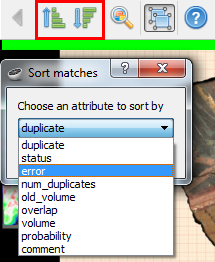
\includegraphics[width=0.30\textwidth]{images/tangerine-sorting.png}
  }\hfill%%%%%%%%%%%%%%%%%%%%%% <========
  \subfloat[Filteren op namen van fragmenten]{
    \label{fig:tangfiltering}
    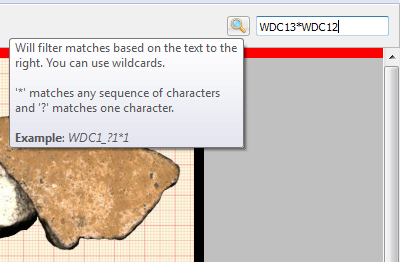
\includegraphics[width=0.60\textwidth]{images/tangerine-namefilter.png}
  }
  \caption{Basis sorteer- en filteroperaties worden via de gebruikersinterface blootgesteld}
  \label{fig:tangfiltersort}
\end{figure}

% \begin{figure}[ht]
%   \begin{minipage}{0.30\textwidth}
%     \centering
%     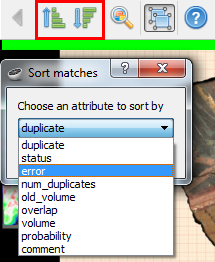
\includegraphics[width=0.60\textwidth]{images/tangerine-sorting.png}
% 	\caption{Sorteren}
% 	\label{fig:tangsorting}
%   \end{minipage}\hfill
%   \begin{minipage}{0.60\textwidth}
%     \centering
%     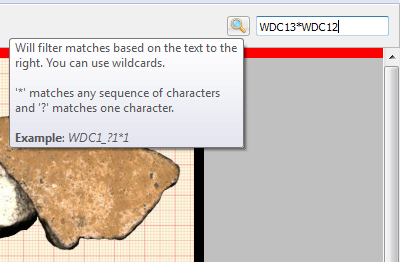
\includegraphics[width=0.60\textwidth]{images/tangerine-namefilter.png}
% 	\caption{Filteren op de namen van de fragmenten}
% 	\label{fig:tangfiltering}
%   \end{minipage}\hfill
% \end{figure}

\subsection{Aanpassingen}
Veranderingen aan de inhoud van de database gebeuren omwille van compatibiliteitsoverwegingen via twee manieren. Globale aanpassingen gebeuren via het model en lokale aanpassingen zoals enkele attributen van een paar gebeuren via het paar zelf. Dit wordt in het volgende hoofdstuk in meer detail besproken.

\section{Modulaire Visualisaties}
Het laatste stuk van de puzzel is de manier waarop de gebruiker met het systeem interageert: de gebruikersomgeving. Deze bestaat uit een schil met daarop een aantal modules die verschillende perspectieven geven op de aanwezige data (meestal onder de vorm van paren). De applicatie (codenaam ``Tangerine'') maakt bij het opstarten de schil aan die de connectie maakt met de databeheerlaag en in staat is verschillende visualisatieplugins te laden (zie figuur~\ref{fig:visualizationlayer}). Dankzij deze flexibiliteit kunnen er in de toekomst met weinig moeite nieuwigheden worden tegevoegd, des te meer omdat visualisatieprototypes zich niet moeten drukmaken om de toevoer van data.\\

De eerste en meest uitgewerkte van de modules werd \emph{MatchTileView} gedoopt, omdat het de paren (\emph{matches}) als tegels laat zien. Dit is dezelfde manier als degene die zo succesvol in het Browsematches prototype werd gebruikt, maar uitgebreid qua mogelijkheiden. De bespreking van de toegevoegde functionaliteiten komt aan bod in het hoofdstuk over modules.\\

\begin{figure}[ht]
	\begin{center}
		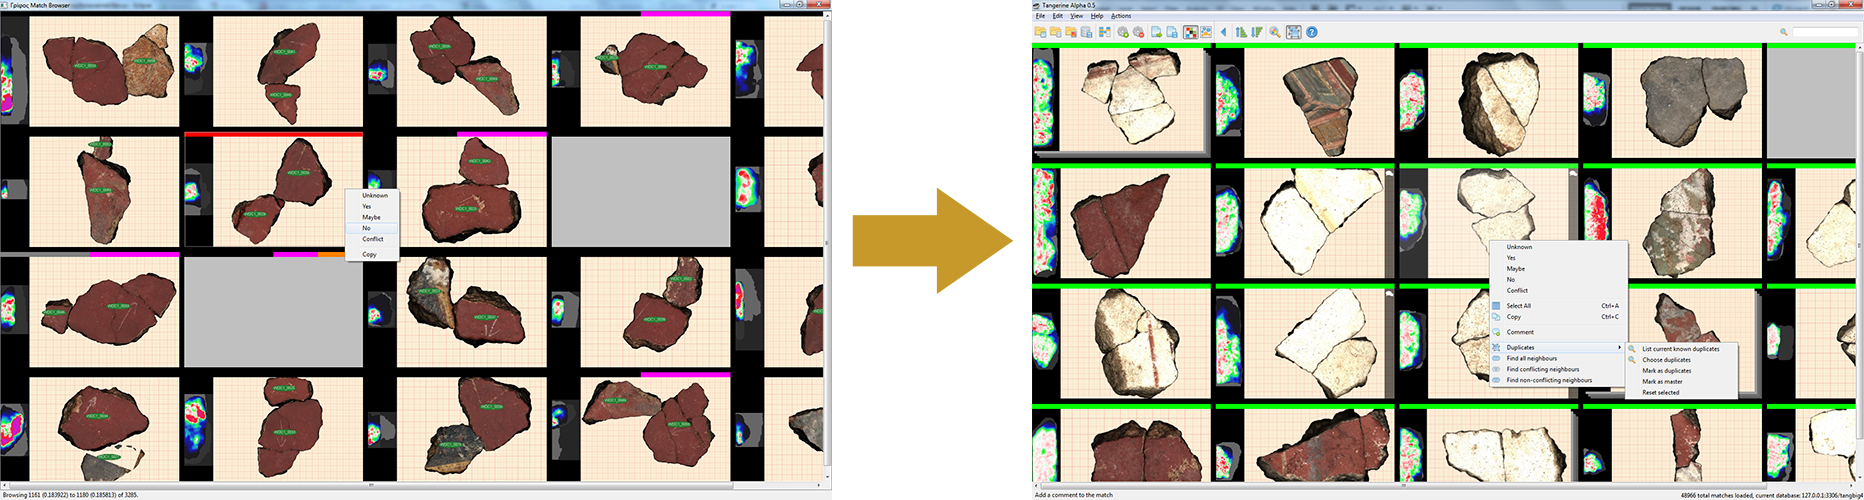
\includegraphics[width=1.0\columnwidth]{images/browsematches-to-tangerine-01.png}
		\caption{De manier van weergeven uit Browsematches werd gekopi\"eerd naar het nieuwe platform, met uitbreidingen}
		\label{fig:browsematchestotang}
	\end{center}
\end{figure}

Elke module krijgt van de applicatie een model toegewezen waar het fragmentparen uit kan opvragen. Dit kan een nieuw model (zonder filters noch sortering) of een gedeeld model zijn. Een gedeeld model behoort niet exclusief tot een module en betekent bijvoorbeeld dat als er \'e\'en beslist om te sorteren op een attribuut zoals ``het verschil van de dikte tussen twee fragmenten'', plots alle modules die gebruikmaken van ditzelfde model over een gesorteerde dataset beschikken. Via speciale signalen worden zij hiervan op de hoogte gebracht, zodat ze kunnen beslissen of het nodig is een actie te ondernemen. Dit kan handig zijn voor pure visualisatieplugins die geen zoekmogelijkheden aan de gebruiker blootstellen, het kan dan vertrouwen op andere modules om data aan te leveren.\\

Indirecte communicatie via het model is (voorlopig) de enige manier waarop modules elkaar kunnen be\"invloeden. De structuur van de componenten ziet er uit als in figuur~\ref{fig:visualizationlayer}. Merk op dat er een plugin is (\emph{DetailView}) die geen gebruik maakt van fragmentparen maar eerder van een virtueel tafelblad net als Griphos. Zoals eerder aangehaald kunnen fragmentparen automatisch op een tafelblad gezet worden. Dit tafelblad kan dan in 3D weergegeven worden door \emph{DetailView}, waarover meer in hoofdstuk~\ref{modules}.

\begin{figure}[h]
	\begin{center}
		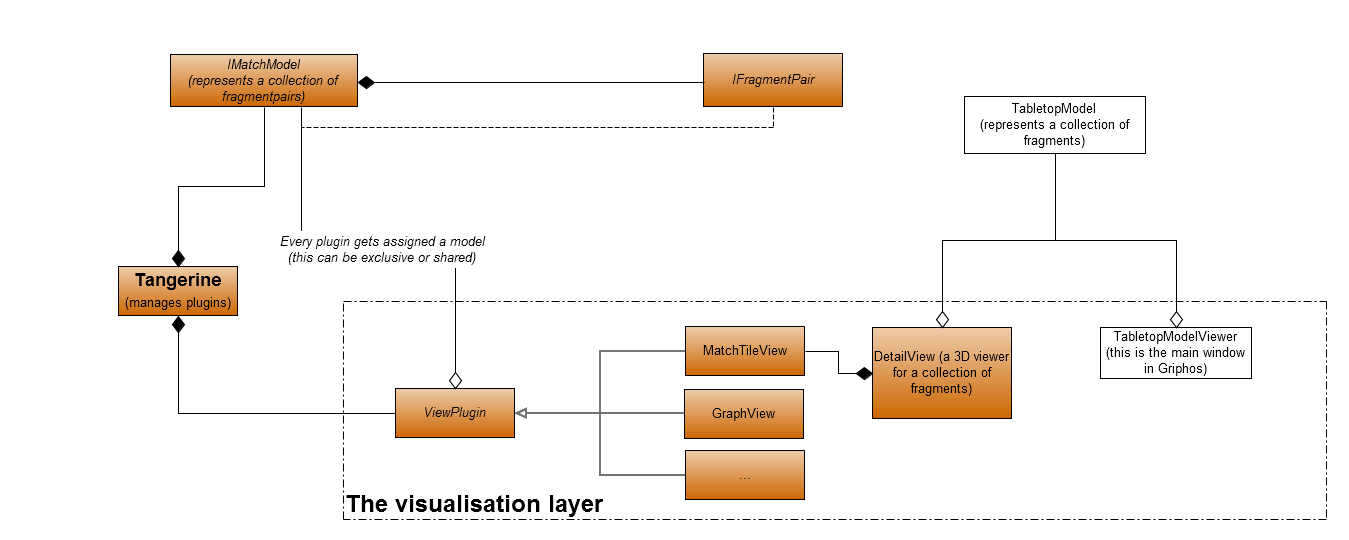
\includegraphics[width=1.0\columnwidth]{images/VisualizationExtract.png}
		\caption{Een vereenvoudigde kijk op de componenten van de visualisatielaag, het hoofdscherm en het model. De componenten in het wit behoren tot de rest van het thera project en zijn niet gemaakt als deel van dit thesisproject.}
		\label{fig:visualizationlayer}
	\end{center}
\end{figure}

\section{Gebruiksgemak / visuele interface}

Vergelijking van wachttijden tussen Griphos/Browsematches en Tangerine

Geheugengebruik BM na grote db: 350 MB (geen afbeeldingen)

Griphos: tonen van een lijst met aparte fragmenten om uit te kiezen (geen equivalent in BM/Tang)
Griphos: tonen van een lijst met alle paren (zoals te zien in figuur~\ldots): 7 minuten 18 seconden <--- NOOT: Griphos gebruikt dezelfde manier van fragmenten inladen als Browsematches, maar laadt ook op voorhand alle afbeeldingen in. Het geheugengebruik na het openenen van 49471 paren is 1.5 GB RAM, het heropenen van dit scherm neemt evenveel tijd in beslag. Het lijkt erop dat het geheugen niet vrijgemaakt noch herbruikt wordt, want bij de tweede keer moest het besturingssysteem het programma afsluiten wegens te veel geheugengebruik.
Browsematches: opstarten en een lijst van alle paren tonen: 49471 paren = 160 seconden en 350MB
Thesisproject: 

% \rowcolors{2}{gray!50}{white}
% \begin{center}
% 	\begin{tabular}{|l|r|r|r|}
% 	    \rowcolor{gray!75}
% 	    \hline
% 	    & \textbf{Griphos} &  \textbf{Browsematches} & \textbf{Thesis (MySQL)} \\
% 	    \hline
% 	    \textbf{Opstartsnelheid} & 1 sec & 16 sec & 1 sec \\
% 	    \textbf{Fragmenten inladen} & 1 min 35 sec  & - & - \\
% 	    \textbf{\textasciitilde 4000 paren laden} & - & 16 sec & 0 sec \\
% 	    \textbf{\textasciitilde 50000 paren laden} & 7 min 18 sec & 2 min 47 sec  & 0-3 sec* \\
% 	    \textbf{\textasciitilde 250000 paren laden} & niet getest & niet getest & 0-15 sec* \\
% 	    \hline
% 	\end{tabular}
% \end{center}


Alle informatie die alleenstaande brokstukken toebehoort --- naam, 3D-voorstelling, contour, \ldots --- wordt opgeslagen als een grote verzameling mappen in het bestandssysteem. Hoewel niet alles meteen wordt ingeladen neemt dit soms toch wat tijd in beslag. Hetzelfde geldt voor een collectie paarvoorstellen waarvan een eerste scherm moet ingeladen worden. Weer een andere bron van vertraging bij het opstarten is het inladen van alle modules, vooral degene die gebruikmaken van OpenGL om fragmenten in 3D weer te geven. Deze stappen  Om deze reden is er voor gezorgd dat deze operaties parallel kunnen lopen, zodat de gebruiker zo weinig mogelijk moet wachten en steeds informatie kan krijgen over de vooruitgang.

De gemiddelde opstarttijd voor Browsematches gemeten op een AMD Athlon X2 5600+ met 2 GB RAM is 10 seconden, waardoor de gebruiker reeds snel gaat denken dat er iets misgelopen is. Bij Browsematches duurde het bijvoorbeeld  is nog  een. 

Alle modules kunnen acties zoals knoppen en menu's  Elk programma dat Bij het initialiseren 

[TODO: verhuizen naar ontwerp van database]
[afbeelding invoegen, selectie naar grafe transit!]\\